\chapter{Volledige ontwerp}
\label{final}
\section{Het finaal ontwerp}
Het finale ontwerp is een 1Mbit geheugen. Het bestaat uit 512 global blocks (GB) en LB met 32 BL en 32 WL. Op elke BL is er plaats voorzien voor één referentie cel. Van de 32 BL worden er 16 gebruikt voor het genereren van het referentiespanning. En van de 16 gebruikte cellen zijn er 6 in HRS en 10 en LRS. Dit om de referentiespanningsverdeling te centreren tussen de BL-spanningen voor cellen in HRS en LRS. De afmetingen van alle transistoren staan in tabel \ref{tab:transsize}. \\
Op dit geheugen wordt een speed-vdd-test uitgevoerd. Dit is een test waarbij de voedingsspanning wordt verlaagd en er vervolgens geverifieerd wordt aan welke snelheid de leescyclus nog kan uitgevoerd worden. Hierbij wordt de dutycycle\footnote{De verhouding van de tijd waarbij de spanningsdeling gebeurd op de totale leestijd. De totale leestijd is de som van de spanningsdelingstijd en de latchingstijd.} spanningsdeling-latching manueel gekozen op basis van het circuitgedrag op de voedingsspanning. Dit geeft natuurlijk een meer optimistisch beeld dan dat er een kloksignaal met een bepaalde frequentie zou verwerkt worden door digitale logica om deze dutycycle te bekomen. De delay van de logica zou overigens niet lineair schalen met de voedingsspanning, waardoor de dutycycle sowieso niet constant blijft. Figuur \ref{fig:speedvdd} toont de resultaten van deze test. Voor elk vakje in de shmoo plot werden 100 Monte Carlo simulaties uitgevoerd, een groen vakje stelt 100 geslaagde leesoperaties voor, bij een rood vakje is er minstens 1 leescyclus foutief verlopen. Zoals men duidelijk kan zien  daalt de leessnelheid bij het verlagen van de voedingsspanning. Dit komt door een combinatie van 2 factoren. Ten eerste wordt de logica trager, dit heeft als gevolg dat de spanningsdeling later wordt uitgevoerd na het schakelen van de controlesignalen. Bovendien komt het signaal aan de gate van de ChargeBL- en DischargeSL-transistor eerder aan dan het WL-signaal. Hierdoor verschijnt er een overshoot bij het laden van de bitlijn zoals in het vorig hoofdstuk werd geillustreerd in figuur \ref{fig:critisch_timing1}. De overshoot treedt eerder op voor LRS-cellen omdat de BL hierbij minder lang moet opladen. Door de overshoot van de BL-spanning moet men langer wachten vooraleer de sense amplifier mag aangezet worden. De tweede factor die de leessnelheid doet vertragen is de SA zelf. Bij een voedingsspanning van 1V kan deze binnen de 0.25ns schakelen. Bij lagere voedingsspanningen kan de SA minder stroom trekken, dit kan in combinatie met mismatch resulteren in een latching van 2ns.

\begin{table}
\begin{center}
\begin{tabularx}{\textwidth}{XXX}
\hline
Transistor & L (nm) & W (nm)\\
\hline
ChargeBL & 195 & 300 \\
DischargeBL & 45 & 100 \\
DischargeSL & 45 & 500 \\
Sa enableP & 45 & 900 \\
Sa enableN & 45 & 500 \\
Sa P & 45 & 1700 \\
Sa N & 45 & 1500 \\
Mux LB & 45 & 200 \\
Mux GB & 45 & 100 \\
\hline
\end{tabularx}
\end{center}
\caption[Transistor afmetingen eind ontwerp]{Afbeeldingen van de transistoren in het eind ontwerp}
\label{tab:transsize}
\end{table}
	
\begin{figure}[!ht]
  \centering
  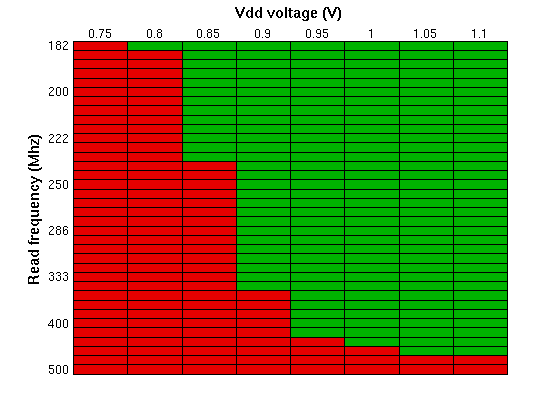
\includegraphics[scale=0.8]{../fig/hfdst-final-vddspeed.png}
  \caption[Resultaten speed-vdd test]{Resultaten speed-vdd test}
  \label{fig:speedvdd}
\end{figure}

Verder kan men ook zien dat de schakeling een voedingsspanning hoger dan of gelijk aan 0.8V nodig heeft om correct te kunnen werken. De verklaring hiervoor kan gezien worden in figuur \ref{fig:vblvdd}. Deze figuur stelt de distributie voor van de BL-spanningen van een cel in RHS, een cel in LRS en de referentiespanning in functie van verschillende voedingsspanningen.Een duidelijke trend bij het verlagen van de voedingsspanningen  is dat deze distributies dichter bij elkaar komen te liggen en dat een voedingsspanning van 0.8V wel degelijk een limiet is. Aangezien de extrema's van de distributies bij een voedingsspanning van 0.8V zo dicht bij elkaar zitten, wordt er verwacht dat de schakeling occasioneel zal falen omdat de SA ontworpen is voor een $\Delta V$ van 35mV. Het incorrect latchen is echter niet geobserveerd bij de 100 Monte Carlo simulaties.
Als men naar de distributies kijkt voor een voedingsspanning van 1V zal men opmerken dat deze niet dezelfde zijn als de distributies getoond in hoofdstuk \ref{loadanalysis}(figuur \ref{fig:distswitch}). De reden hiervoor is dat men in de speed-vdd-test niet wacht tot de bitlijn volledig is opgeladen, wat een tijdswinst oplevert. Ook werd er in hoofdstuk \ref{loadanalysis} gesuggereerd dat een energiewinst zou bereikt kunnen worden door een andere last te kiezen (sectie \ref{anderelast}). Hoewel dit mogelijk is, heeft dit wel als nadeel dat de schakeling minder tolerant is voor voedingsspanningvariaties. Tenslotte moet ook vermeld worden dat de speed-vdd-test uitgevoerd werd op een (SPICE) temperatuur van $30^{\circ}\mathrm{C}$. Moest deze schakeling worden geïmplementeerd in een processor is de kans groot dat dit onderhevig zal zijn aan temperaturen tussen de $-40^{\circ}\mathrm{C}$ en $85^{\circ}\mathrm{C}$ wat ook tragere leessnelheden zal opleveren. Hoe traag werd echter niet onderzocht.

\begin{figure}[!ht]
  \centering
  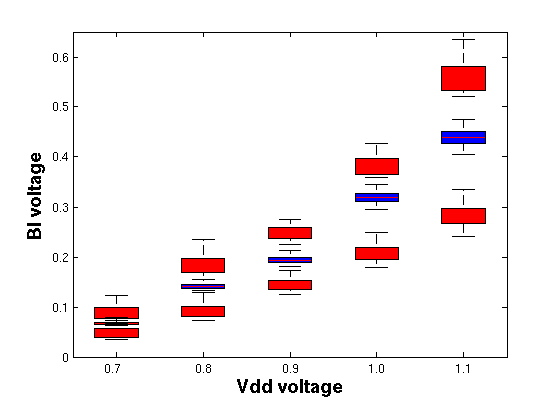
\includegraphics[scale=0.8]{../fig/hfdst-final-vddbl.png}
  \caption[Bl-spanningen i.f.v. Vdd]{Bl-spanningen voor Referentie, HRS en LRS i.f.v. Vdd}
  \label{fig:vblvdd}
\end{figure}

Het totale energieverbruik van een leescyclus bij een voedingsspanning van 1V is gemiddeld 0.51pJ. Hierbij gaat 25\% van de energie naar de logica, 2\% naar de sense amplifier, 65\% naar de stroomdeling en 8\% naar de buffers. Hierbij werden de decoderbuffers bij logica gerekend.

\section{Vergelijking met de literatuur}
Het vergelijken van 2 geheugens is geen evidentie. Ten eerste verschillen vaak de vooropgestelde chipspecificaties, ten tweede verschillen vaak de technologieën en tenslotte geven veel papers niet alle resultaten weer om goed te kunnen vergelijken. Chipspecificaties hangen af van de noden van de applicatie van de chip. Voor automotive applicaties bijvoorbeeld is er vooral nood aan geheugens die bij hoge temperaturen een hoge betrouwbaarheid hebben. Medische toepassingen daarentegen hebben  nood aan low-power chips. Onder verschillende technologieën kan er een onderscheid gemaakt worden tussen de technologie van de logica en van het geheugen. Zo wordt er vaak voor verschillende toepassingen een andere soort NOR-flash geheugencel gebruikt: charge-trapping-cellen worden gebruikt voor betere betrouwbaarheid, split-gates-cellen voor hoge performantie \cite{5783209}. De schakeling ontworpen in dit werk kan bij de snellere geheugens worden gecategoriseerd wanneer men vergelijkt met NOR-geheugens in de industrie \cite{6649105}\cite{4433985}\cite{4027813}. Hierbij werd er gekeken naar de random-access-leessnelheid. Vaak kan een groot verschil in leessnelheid (gedeeltelijk) verklaard worden door de bitlijncapaciteit. \\ 
Energieverbruik kan berekend worden d.m.v $CV_{vdd}^{2}$. Meestal wordt energieverbruik niet vermeld in papers maar gezien de lage voedingsspanning bij 45nm technologie, kan men vermoeden dat de schakeling in dit werk ook bij de meer energiezuinige schakelingen hoort. De meeste schakelingen gevonden in de literatuur hebben namelijk een hogere voedingsspanning. De werking van het ontworpen RRAM geheugen op verschillende temperaturen werd in dit werk niet onderzocht. Naast verschillen in de werking van de logica zal ook de memristor onderhevig zijn aan temperatuursveranderingen. Volgens \cite{5948374} zal bij een $HfO_{2}$ geheugencel de $R_{OFF}/R_{ON}$-verhouding dalen bij stijgende temperatuur. Ondanks deze daling in performatie ziet men in de industrie toch RRAM-chips opduiken die functioneren bij hoge temperaturen\footnote{http://www.crossbar-inc.com/markets/automotive.html}. Men kan besluiten dat met de afbakening in het achterhoofd de schakeling een goede prestatie levert t.o.v. schakelingen in de literatuur.

\section{Besluit}
Een finale schakeling werd ontworpen en geëvalueerd. Hierbij werd er voornamelijk gekeken naar de prestatie onder verschillende voedingsspanningen. Er werd een absolute limiet van minimum 0.8V gevonden voor de voedingsspanning en verklaard. Verder werd een vergelijkende studie uitgevoerd met NOR-flash schakelingen in de literatuur en op basis hiervan werd er besloten dat de schakeling in dit werk een goed alternatief is op het vlak van snelheid en energieverbruik. Andere aspecten kunnen niet vergeleken worden aangezien deze niet onderzocht werden in dit werk.
